\chapter{\textsc{Background and related work}} 

This chapter focuses on background and related work from academic and non-academic sources. Gaps of current studies are identified, and at the end of the chapter, contributions of the author's work are proposed.

\section{IACS overview}


IACS elements are distributed in so-called \gls*{ot} network. \gls*{ot} networks are distinguished between conventional \gls*{it} systems as \gls*{ot} systems run a time-critical process where the smallest delay can cause system disruption. Research \parencite{77-ics-kill-chain} has summarized differences as displayed in the table \ref{tab:it-vs-ot}.

\begin{longtable}[c]{|p{0.2\textwidth}|p{0.35\textwidth}|p{0.4\textwidth}|}
	\caption{\raggedright{Difference between traditional IT system and IACS \parencite{77-ics-kill-chain}.}}
	\label{tab:it-vs-ot}\\
	\hline
	\textbf{Item}           & \textbf{IT System}                                    & \textbf{IACS}                                                                                                                                                     \\ \hline
	\endfirsthead
	%
	%\multicolumn{3}{c}%
	%{{\bfseries Table \thetable\ continued from previous page}} \\
	\hline
	\textbf{Item}           & \textbf{IT System}                                    & \textbf{IACS}                                                                                                                                                     \\ \hline
	\endhead
	%
	Operating Systems (OS)       & General purpose OS (MS Windows, Linux, Unix)             & Embedded OS (VxWorks, uClinux etc.), General purpose OS with reduced functionality.                                                                               \\ \hline
	Data exchange protocols & TCP / IP protocol stack                               & Field-specific proprietary and open-source protocols (DPN3, Modbus, OPC etc.) are used as an application layer of the TCP / IP stack or via the serial communication bus. \\ \hline
	Real-time requirements & Low requirements for real-time data roundtrips        & High requirements for real-time data round-trips, delays, or disruptions can be damaging.                                                                          \\ \hline
	System fault response   & Response level dependent on IT system requirements    & Interruption can cause financial and physical loss.                                                                                                               \\ \hline
	System upgrades         & Almost all the systems are relatively easy to upgrade. & Due to poor hardware compatibility, upgrades usually are not advised.                                                                                               \\ \hline
	
\end{longtable}


The common components making up an IACS system are as follows \parencite{30-rewiev-of-all-testbeds2020}: 

\begin{itemize}
	\item \gls*{plc};
	\item \gls*{hmi};
	\item \gls*{scada} workstations;
	\item \gls*{ied};
	\item \gls*{rtu};
	\item Data historians.
\end{itemize}

The main control elements in a cyber-physical system are usually \gls*{plc}, which receives external inputs, performs a logic operation, and acts on outputs accordingly. The high-level process of \gls*{plc} is shown in figure \ref{fig:plc-operation}.

\begin{figure}
	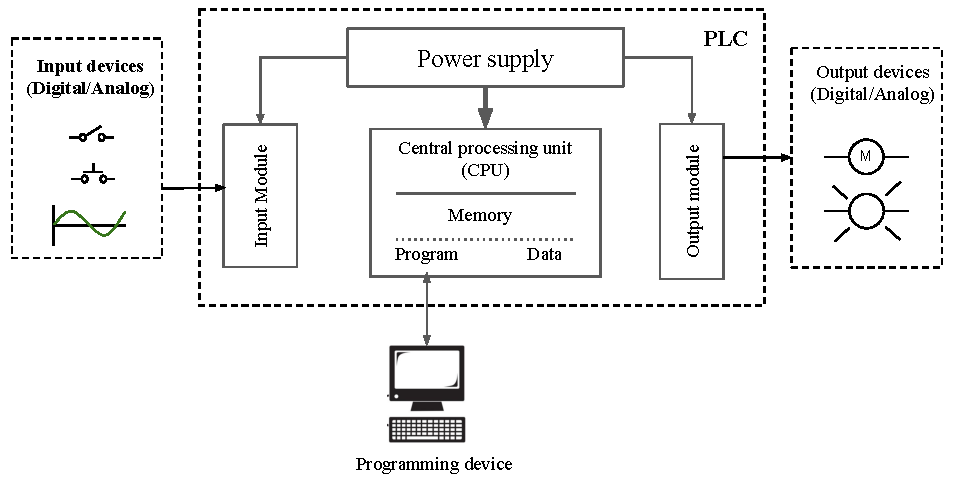
\includegraphics[width=\linewidth]{plc-structure.pdf}
	\caption{High level overview of \gls*{plc} operation  \parencite{97-siemens-plc-intro}.}
	\label{fig:plc-operation}
\end{figure} 

PLC is a programmable device. Nowadays, the programming of PLC is performed by general purpose PC, which runs programming software. Programs usually can be created in five standardized IEC61131-3 languages \parencite{WEB-14-plc-languages}: 

\begin{itemize}
	\item \gls*{lad} - graphical language, which imitates the behavior of electromechanical relay contacts. It was common in early automation designs. LAD can also perform more sophisticated operators as implementing timers, counters, cooperators, mathematical functions, moving operations of memory segments, signal conversions, etc.;
	
	\item \gls*{fbd} - graphical language, where chained function blocks visualize the logic decision flow from one block to another;
	
	\item \gls*{scl} - text-based programming language which is derived from pascal;
	
	\item \gls*{sfc} - graphical block diagram-based language where the program is structured as a flowchart;
	
	\item \gls*{il} - text-based programming language which closely resembles assembler. It is mostly used for compact and time-critical programs.
\end{itemize}

Program for PLC is compiled for the actual hardware of the PLC that will control the physical process. Thus, the control layer is mapped to the cyber-layer, and it exists in actuality as a compiled program in binary machine code. It resides in the memory of the PLCs hardware and is processed by the CPU of the hardware. In the real system, the PLC is connected to actuators and sensors that operate a physical process \parencite{WEB-04-plc-vendors}. This can be seen in figure \ref{fig:plc-operation}.

Visualization in IACS is done by a \gls*{hmi} or \gls*{scada}. \gls*{hmi} is usually a purpose-built physical PC with a built-in display to visualize the physical process and allows for the operator to interact with the process. \gls*{scada} typically is computer software installed on a general-purpose PC or server that allows the operator to oversee the physical process and interact with it. SCADA also can be used to collect and visualize the data from geographically distributed control systems.

It is worth mentioning that the term SCADA is often used misleading as SCADA is usually computer software installed on a workstation, allowing the operator to monitor and interact with the system. SCADA workstations can be installed locally or in a wide area like an electrical grid. Wide-area SCADA has more components to allow connections to remote sites, including RTUs, which serve as information gateways between end devices and SCADA workstations. Thus, when research usually mentions SCADA, it means SCADA networks with vastly interconnected field devices which send data to the central control center.

According to research \parencite{48-red-tee-ics-testbed} IACS security is a significant challenge. Firstly, the complexity and diversity of devices involved in the IACS increase the attack surface. For example, an attacker might strike the cyber-part, the physical part, or both parts of the IACS.

As indicated by \citeauthor{29-ICS-cyber-range-scenarios} \parencite{29-ICS-cyber-range-scenarios} 
until 2020, 60\% of manufacturing companies have been subject to cyberattacks, and almost a third of them suffered financial loss and, as a result, disruption of the business.

\citeauthor{48-red-tee-ics-testbed} \parencite{48-red-tee-ics-testbed} express a point of view that the issues in IACS security results from the interdisciplinary nature of the problem. It is challenging to bring together experts from different fields, such as information security, information technologies, and automation engineering.

\section{Literature review} \label{sec:lit-rev}

This section will look at the overall research done on IACS testbeds, and afterwards, describe CRs with regards to architecture, objectives, purpose, and design considerations.
 

The systematic literature review aims to identify and evaluate the existing literature of scientific research regarding a particular research question or topic.

The objective of this literature review is to study the concepts, trends, architecture, and scenarios of previous research to determine shortcomings in the field of IACS CRs.

For the search of scientific articles, the author has used the following keywords: \textit{ IACS/ICS testbeds, IACS/ICS testbed reviews, SCADA cybersecurity testbed, IACS cyber range }. The author used IEEE and Scopus scientific databases and Google Scholar search engines to search for literature. As the IACS field develops quickly, five year period was chosen as an optimal time frame for literature review. Found papers were reviewed, and approximately 40 relevant articles and ten cited in these articles were deemed relevant and read through thoroughly.

\subsection{Overview of current IACS cyber ranges}

IACS systems usually are critical systems that cannot be offline or face failures during their operation. Thereby, \citeauthor{02-surway} \parencite{02-surway} points out that the high availability requirements on IACS do not allow performing security tests on a live system. \citeauthor{09-iiot-testbed-architecture} \parencite{09-iiot-testbed-architecture} presents a point that there is a lack of knowledge about the attack surfaces of overlapping OT/IoT/IT systems, possible vulnerabilities, and defense mechanisms that may mitigate risks of attacks to such overlapping systems. For this reason, researchers, corporations, and military institutions turn to cyber ranges that mimic real IACS.

\citeauthor{29-ICS-cyber-range-scenarios} \parencite{29-ICS-cyber-range-scenarios} state that developing cyber-security competencies through the use of \gls*{cr} and their use for research topics is of increasing interest. In addition, CR is a tool that can help improve the stability, security, and performance strength of IT/OT systems. Also, CRs are a vital tool for exploring and modeling vulnerabilities, and producing viable data sets that enable testing security solutions as novel architectures, intrusion detection systems, and attacks against infrastructure.

According to the literature review, 28 created testbeds were found in the relatively new research. These testbeds are indicated in table \ref{tab:testbed-owerview-countries-years}.

% Please add the following required packages to your document preamble:
% \usepackage{longtable}
% Note: It may be necessary to compile the document several times to get a multi-page table to line up properly
\begin{longtable}[c]{|c|c|c|c|c|c|p{0.25\textwidth}|}
	\caption{\raggedright{Cyber range overview (Chemical plant - C, Smart Grid - SG, Nuclear plant - N, General - G, Electrical Grid - G, Transportation - T, Manufacturing - M, Water Treatment - W).}}
	\label{tab:testbed-owerview-countries-years}\\
	\hline
	\textbf{Nr.} & \textbf{Name} & \textbf{Country} & \textbf{Year} & \textbf{Field} & \textbf{Type} & \textbf{Ref.}                                      \\ \hline
	\endfirsthead
	\hline
	\textbf{Nr.} & \textbf{Name} & \textbf{Country} & \textbf{Year} & \textbf{Field} & \textbf{Type} & \textbf{Ref.}                                      \\ \hline
	\endhead
	%
	1            & n/a           & USA              & 2012          & G              & V             & \cite{03-testbeds}                                 \\ \hline
	2            & n/a           & USA              & 2017          & EG             & V             & \cite{04-virtual-testbed}                          \\ \hline
	3            & n/a           & USA              & 2016          & EG             & P             & \cite{05-testbeds}                                 \\ \hline
	4            & VTET          & China            & 2018          & C              & H             & \cite{06-testbed}                                  \\ \hline
	5            & n/a           & Qatar           & 2021          & C              & H             & \cite{07-testbed-methadology}                      \\ \hline
	6            & n/a           & USA              & 2019          & N, T           & P             & \cite{10-testbed-research}                         \\ \hline
	7            & n/a           & USA              & 2017          & G              & P             & \cite{12-ICS-testbed}                              \\ \hline
	8            & MSICST        & China            & 2019          & G              & P             & \cite{13-experiences-in-ICS-testbeds}              \\ \hline
	9            & n/a           & Portugal         & 2017          & EG             & V             & \cite{15-testbed-SCADA-atack}                      \\ \hline
	10           & n/a           & USA              & 2019          & C              & P             & \cite{17-SCADA-testbed}                            \\ \hline
	11           & IOSB          & Germany          & 2017          & M              & H             & \cite{22-ICS-testbed-design-and-architect}         \\ \hline
	12           & EPIC          & Singapore        & 2019          & SG             & P             & \cite{25-testbed-EPIC}                             \\ \hline
	13           & n/a           & France           & 2017          & EG             & P             & \cite{26-springer-testbeds}                        \\ \hline
	14           & n/a           & Netherlands      & 2018          & EG             & V             & \cite{27-integrated-testbed-for-SCADA-monitoring}  \\ \hline
	15           & n/a           & Switzerland      & 2018          & T              & V             & \cite{28-testbed-road-infra}                       \\ \hline
	16           & n/a           & USA              & 2021          & HVAC           & V             & \cite{31-springer-plc-and-iot-in-virtual-testbed}  \\ \hline
	17           & RICS-el       & Sweden          & 2019          & EG             & V             & \cite{32-springer-scada-testbed-research-training} \\ \hline
	18           & n/a           & USA              & 2018          & G              & V             & \cite{33-SCADA-virtual-testbed}                    \\ \hline
	19           & SWAT          & Singapore        & 2016          & W              & P             & \cite{34-ieee-swat-ics-testbed}                    \\ \hline
	20           & PowerCyber    & USA              & 2010          & EG             & n/a           & \cite{36-SCADA-testbeds-2010}                      \\ \hline
	21           & GRFICS        & USA              & 2018          & C              & V             & \cite{39-grfics-scada-simulator}                   \\ \hline
	22           & n/a           & Italy            & 2010          & EG             & H             & \cite{40-scada-testbed}                            \\ \hline
	23           & VCSE          & USA              & 2011          & EG             & V             & \cite{41-vcse-ics-testbed}                         \\ \hline
	24           & n/a           & USA              & 2011          & G              & P             & \cite{43-SCADA-testbed-for-protection-concepts}    \\ \hline
	25           & VPST          & USA              & 2009          & EG             & V             & \cite{46-VPST-testbed-2009}                        \\ \hline
	26           & TASSCS        & USA              & 2011          & EG             & V             & \cite{47-ieee-tasscs-testbed}                      \\ \hline
	27           & ICSrange      & Italy            & 2019          & G              & V             & \cite{48-red-tee-ics-testbed}                      \\ \hline
	28           & SoftGrid      & Singapore        & 2016          & EG             & V             & \cite{50-softgrid-scada-testbed}                   \\ \hline
	
\end{longtable}


Table \ref{tab:testbed-owerview-countries-years} shows that half of the testbeds are created in the USA, and the rest are scattered across Europe and Asia. However, in recent years, the number of CRs and testbeds is increasing in Europe and Asia. In the author's opinion, the increase of IACS CR research topics is explained by developments in the IACS field where OT systems merge with IT networks. 

IACS CR typical applications include electrical generation plants, the chemical and oil industry, water and wastewater management, nuclear power stations, and the manufacturing industry. The primary industry created in CRs is energy transmission and generation. In author's opinion, the energy sector is one of the most obvious targets for adversaries as nowadays everything relies on electricity. Secondly, research using an electrical grid can more easily emphasize the gravity of cyberattacks. 

\citeauthor{17-SCADA-testbed} \parencite{17-SCADA-testbed} shows that a literature vacuum exists about detailed cyber range documentation, focusing on cyber-security readiness, penetration testing, IACS protocols analysis, vulnerability assessments, defensive and offensive security, risk analysis, and IACS incident forensics.

CRs use different vendor elements and protocols in their systems. All of this data is collected in table \ref{tab:testbed-owerview-vendors}. One of the most common vendors used in physical IACS cyber ranges across multiple studies are Siemens and Allen-Bradley.  In author's opinion popularity of these vendors can be justified by vendor presence in worldwide markets and across virtually all industries.

% Please add the following required packages to your document preamble:
% \usepackage{longtable}
% Note: It may be necessary to compile the document several times to get a multi-page table to line up properly
\begin{longtable}[c]{|c|l|p{0.18\textwidth}|p{0.25\textwidth}|p{0.22\textwidth}|}
	\caption{\raggedright{IACS testbed overview by vendors and protocols.}}
	\label{tab:testbed-owerview-vendors}\\
	\hline
	\textbf{Nr.} & \textbf{Name} & \textbf{Vendors}                & \textbf{Protocols}                             & \textbf{Ref.}                                      \\ \hline
	\endfirsthead
	%
	%\multicolumn{6}{c}%
	%{{\bfseries Table \thetable\ continued from previous page}} \\
	\hline
	\textbf{Nr.} & \textbf{Name} & \textbf{Vendors}                & \textbf{Protocols}                             & \textbf{Ref.}                                      \\ \hline
	\endhead
	%
	1            & n/a            & n/a                              & n/a                                            & \cite{03-testbeds}                                 \\ \hline
	2            & n/a             & n/a                              & Modbus/TCP                                         & \cite{04-virtual-testbed}                          \\ \hline
	3            & n/a           & n/a                              & n/a                                            & \cite{05-testbeds}                                 \\ \hline
	4            & VTET          & Siemens                          & OPC, Modbus/TCP, S7comm                            & \cite{06-testbed}                                  \\ \hline
	5            & n/a          & Siemens                          & Profinet                                       & \cite{07-testbed-methadology}                      \\ \hline
	6            & n/a           & n/a                              & Modbus/TCP                                         & \cite{10-testbed-research}                         \\ \hline
	7            & n/a          & Siemens                          & Profinet                                       & \cite{12-ICS-testbed}                              \\ \hline
	8            & MSICST        & Siemens, Rockwell, GE, Schneider & S7comm, EDG, Modbus/TCP                           & \cite{13-experiences-in-ICS-testbeds}              \\ \hline
	9            & n/a           & n/a                              & Modbus/TCP                                         & \cite{15-testbed-SCADA-atack}                      \\ \hline
	10           & n/a           & Multiple                         & Modbus/TCP, OPC, ARTI, DNP3, KOYO, IEC 60870-5-104 & \cite{17-SCADA-testbed}                            \\ \hline
	11           & IOSB          & Siemens                          & S7comm, OPC, Profinet                          & \cite{22-ICS-testbed-design-and-architect}         \\ \hline
	12           & EPIC          & Multiple                         & IEC-61850, Modbus/TCP                              & \cite{25-testbed-EPIC}                             \\ \hline
	13           & n/a          & Multiple                         & Modbus/TCP, DNP3                                   & \cite{26-springer-testbeds}                        \\ \hline
	14           & n/a           & n/a                              & Modbus/TCP                                         & \cite{27-integrated-testbed-for-SCADA-monitoring}  \\ \hline
	15           & n/a           & n/a                              & Modbus/TCP                                         & \cite{28-testbed-road-infra}                       \\ \hline
	16           & n/a           & OpenPLC                          & n/a                                            & \cite{31-springer-plc-and-iot-in-virtual-testbed}  \\ \hline
	17           & RICS-el       & n/a                              & IEC 60870-5-104                                & \cite{32-springer-scada-testbed-research-training} \\ \hline
	18           & n/a           & n/a                              & Modbus/TCP, DNP3                                   & \cite{33-SCADA-virtual-testbed}                    \\ \hline
	19           & SWAT          & Allan-Bradley's                 & EtherNet/IP, CIP                               & \cite{34-ieee-swat-ics-testbed}                    \\ \hline
	20           & PowerCyber    & n/a                              & DNP3, IEC 61850                                & \cite{36-SCADA-testbeds-2010}                      \\ \hline
	21           & GRFICS        & n/a                              & n/a                                            & \cite{39-grfics-scada-simulator}                   \\ \hline
	22           & n/a           & ABB, OpenPLC                     & Modbus/TCP, DNP3                                   & \cite{40-scada-testbed}                            \\ \hline
	23           & VCSE          & n/a                              & n/a                                            & \cite{41-vcse-ics-testbed}                         \\ \hline
	24           & n/a           & Multiple                         & Modbus/TCP, DNP3                                   & \cite{43-SCADA-testbed-for-protection-concepts}    \\ \hline
	25           & VPST          & n/a                              & DNP3                                           & \cite{46-VPST-testbed-2009}                        \\ \hline
	26           & TASSCS        & n/a                              & DNP3, Modbus/TCP                                   & \cite{47-ieee-tasscs-testbed}                      \\ \hline
	27           & ICSrange      & n/a                              & Multiple                                       & \cite{48-red-tee-ics-testbed}                      \\ \hline
	28           & SoftGrid      & n/a                              & IEC 60870, IEC61850                            & \cite{50-softgrid-scada-testbed}                   \\ \hline
	
\end{longtable}

As the crucial part of the IACS system lies in the communication between control elements, TCP/IP communication protocols are used, which is also one of the broad attack surfaces of IACS. In table \ref{tab:testbed-owerview-vendors} used protocols are listed, and one of the most used protocols in cyber ranges across multiple fields of IACS is Modbus. It is widely used because the protocol is open-source with vastly available documentation and relatively easily exploitable vulnerabilities. Another protocol of interest is \gls*{dnp3}, which is mainly utilized in electric and water utilities mainly in the USA. \gls*{s7} is a Siemens proprietary protocol used in communication between PLCs of the Siemens S7-300/400/1200/1500 family. \gls*{opc} is a series of standards and specifications for industrial telecommunication, mainly used in higher-level management systems.  

Testbeds and CRs can be divided by type, purpose, and supporting sector. Sectors are academic, military, or commercial. Most of the reviewed research is about CRs in the academic sector. Regarding purpose, CRs are divided into flowing parts: team building, cyber training, capture the flag events, research and development, testing, assessment, and recruitment. The broad spectrum of purposes requires an extensible and configurable IACS platform. Multiple researches \parencite{03-testbeds, 01-surway} divide CRs by physical, virtual, and hybrid architecture. Many testbeds hybridize the physical and virtual components to make a trade-off between fidelity and economy, which is also confirmed by table \ref{tab:testbed-owerview-countries-years}. Most research is done on virtualized testbeds as they are cheap and relatively easy to implement and re-purpose. Further, these three CR architectures are described in detail.

\subsubsection{Physical testbed} \label{ss:physical-testbed}

This type of testbeds uses physical hardware and actual software running on hardware. Some of the physical CRs as \parencite{25-testbed-EPIC, 34-ieee-swat-ics-testbed} are used to control the actual physical process containing actuators and sensors. Despite the advantages, most physical CRs use the \gls*{hil} physical system simulation method, which uses mathematical models to represent the physical process. There is a lack of exact mathematical models for representing the behaviors of sensors and actuators used in monitoring and controlling the physical devices. \citeauthor{35-ten-lessons-ics-testbeds} \parencite{35-ten-lessons-ics-testbeds} points out HIL is not that necessary as these mathematical models cannot reproduce the exact physical model. Hence simple physical stimulation can be enough.

One of such physical CR is \gls*{swat} \parencite{34-ieee-swat-ics-testbed}. \gls*{swat} consists of a six stage water treatment process, each stage is autonomously controlled by a local PLC. As indicated by \citeauthor{01-surway} \parencite{01-surway} this testbed framework is widely used in many research papers, for instance, \citetitle{swat-ref-02} \parencite{swat-ref-02}, \citetitle{swat-reference-01} \parencite{swat-reference-01}.

Most of the reviewed research agrees that physical CRs closely represent real-life system, suggesting that it has the highest fidelity. It can contain hardware, firmware, and software vulnerabilities, thus exposing a broader attack surface to exploit. In this way, it allows to understand attacker incentives better.

Possible drawbacks of such physical CRs are:

\begin{itemize}
	\item Difficulty to reconfigure and maintain real hardware and software in a testbed, especially given the presence of firmware exploits that have the potential to damage elements;
	
	\item Difficulty for researchers to build large-scale CRs due to cost limitations. Therefore, researchers usually use a small amount of necessary core physical components to build a minimal IACS test environment and surround it with virtualized components.
	
\end{itemize}

However, \citeauthor{03-testbeds} \parencite{03-testbeds} imply that physical testbeds have several advantages compared to virtual systems:

\begin{itemize}
	\item Data reflect realistic measurement variations that would be present in an actual process control system;
	
	\item Communication patterns and latency is entirely accurate and not vulnerable to inaccuracies in simulated variables like OS scheduling load;
	
	\item  IACS elements can hold software, firmware, and hardware vulnerabilities which is not possible for virtual testbeds. These attacks can be provided in addition to protocol-based attacks.
\end{itemize}

\subsubsection{Virtualized testbed} \label{subsec:virtual}

\citeauthor{06-testbed} \parencite{06-testbed} mentions that virtualization of the testbed is a straightforward approach to overcome the disadvantages mentioned in section \ref{ss:physical-testbed} Although the virtual testbed would lose some fidelity, it is more suitable for preliminary IACS security research in the laboratory environment. 

\citeauthor{01-surway} \parencite{01-surway} illustrates that the virtualized testbed enables researchers to conduct low-cost, reusable security studies in a real IACS configuration environment with an IT architecture. However, virtualized complex physical processes involve a large amount of computation. Therefore the hardware requirements of the computer are high. As an advantage, virtual CRs have high scalability and generally operate on either a single or a small number of servers.  Additionally, virtualization can only support open-source PLCs and related software in virtual machines. On the downside, mainstream PLCs, such as, Schneider, Omron, and Siemens are closed-source industrial devices. Commercial vendors have limited information on hardware and firmware, making it difficult to virtualize these PLCs. So one of the biggest obstacles to virtualize high-fidelity IACS testbeds is the lack of open-source virtualized PLCs.  For virtualization purposes, the OpenPLC controller is used \parencite{38-ieee-openplc.pdf}. OpenPLC supports five programming languages based on IEC61131-3 \parencite{WEB-14-plc-languages} and commonly used IACS protocols - Modbus TCP, DNP3 and others. Therefore OpenPLC is easy to deploy and relatively cheap to install and maintain. However, several academic papers question whether test results from a simulation reflect reality.

One of such virtualized testbed is GRFIACS framework \parencite{39-grfics-scada-simulator} based on OpenPLC \parencite{38-ieee-openplc.pdf} research. The framework was created relatively recently in the year 2018. GRFIACS virtualized the entire IACS network and physical processes. The GRFIACS testbed can be used to practice common methods of IACS attacks and exploits while observing the impact of network attacks on physical processes.

Advantages mentioned by \citeauthor{03-testbeds} \parencite{03-testbeds} are:

\begin{itemize}
	\item Virtual testbeds are easy to duplicate and reproduce. Virtual testbed platform reduces duplication of effort as research groups do not have to develop testbeds from scratch. An open platform enables researchers to update existing virtual testbeds;
	
	\item Virtual testbed platform provides a common ground for research enabling research groups to share code and enabling published results to be duplicated and compared.
	
\end{itemize}


\subsubsection{Hybrid testbed} \label{subsec:hybrid-testbed}

Hybrid testbeds try to combine the best of both worlds, virtual and physical. Testbed by this approach can be created using physical components, such as, PLCs, HMIs, and other physical systems that are hard or close to impossible to virtualize or simulate. On the other hand, system elements like SCADA workstations, historians, and network infrastructure can be virtualized. For example, SCADA commonly resides on MS Windows type of operating system that can be run in a virtual environment like VMware or VirtualBox.

One of such CR was created by \citeauthor{15-testbed-SCADA-atack} \parencite{15-testbed-SCADA-atack}. The study created an electrical grid CR where SCADA and the network ran in a virtual environment, but elements controlling circuit breakers and disconnectors were physical devices. \citeauthor{15-testbed-SCADA-atack} mentions that this setup provides more information about less evident events in the SCADA system during attacks.

\citeauthor{22-ICS-testbed-design-and-architect} \parencite{22-ICS-testbed-design-and-architect} has created a CR by dividing in physical and virtual parts as follows:

\begin{itemize}
	\item Virtualization environment - virtual switches, VM PLC programming stations, VM SCADA servers, attack detection tools;
	
	\item Physical environment - PLCs, industrial actuators, HMIs, RTUs.
\end{itemize}

\subsection{Objectives, purpose, and requirements of IACS cyber ranges} \label{subsec:objectives-purpose-reqeurements}

Researches \parencite{13-experiences-in-ICS-testbeds, 20-dsign-and-realization-of-testbeds} mention that the testbed and cyber ranges can be built for a multitude of purposes such as vulnerability analysis, education and training, tests of defense mechanisms, control system tests, performance analysis, honeypot, impact analysis, threat analysis, and creation of standards. However, review by \citeauthor{42-surway-australi-unclasified} \parencite{42-surway-australi-unclasified} argues that CRs are predominantly used for training. The training varies in complexity going from computer security fundamentals to advanced \gls*{ttp} for \gls*{cno}. As described in NIST Glossary \parencite{WEB15-nist-glosary} \gls*{ttp} are adversary behaviors where tactics are high-level actions and techniques are behaviors attacker performs in the context of the specific technique. Term \gls*{cno} encapsulates defense and offense computer operations.

Diversity in the range of IACS elements, software, and protocols, is essential to replicate real-world scenarios in cyber ranges. \citeauthor{35-ten-lessons-ics-testbeds} \parencite{35-ten-lessons-ics-testbeds} points out that diversity comes at a cost, not only in financial terms but also with regards to scalability and complexity of the experimental infrastructure.

Researches are aiming for low cost and still keeping some fidelity of IACS cyber range to develop CRs with physical and virtual components, making them hybrid testbeds. Physical elements are the ones increasing the fidelity of the system. One such CR was created by \citeauthor{06-testbed} \parencite{06-testbed} it is Virtual Tennessee-Eastman Testbed (VTET) which consists of virtual and physical elements. \citeauthor{20-dsign-and-realization-of-testbeds} \parencite{20-dsign-and-realization-of-testbeds} mentions that it is essential to understand which components are required to be real and which should be virtual. This is undoubtedly one of the most important decisions when designing a testbed for security research. Several trade-offs have to be considered depending on the individual project scope, domain, and intended research.

CR requirements change based on objectives. For example, \citeauthor{39-grfics-scada-simulator} in research \parencite{39-grfics-scada-simulator} has created GRFIACS testbed framework, which is intended to help beginners in IACS security to overcome barrier created by the exclusive use of expensive, proprietary hardware and software used in IACS. CR is designed for students to create an attack that causes significant physical damage to the simulated system. Therefore, \citeauthor{39-grfics-scada-simulator} as main requirements mention modular design to allow swapping virtual elements with physical ones, low initial cost, and simple communication protocols for students to reduce the learning curve. Other researches as \parencite{40-scada-testbed, 04-virtual-testbed} have created electrical grid hybrid IACS cyber rages. In this case, the main objective of the research was to understand the cascading effects of failures in IACS with realistic attack scenarios and to test novel cyber-attacks. These testbeds require sophisticated simulation of the electrical grid to understand the impact of attacks. Thus, minor emphasis is placed on control system complexity.


From reviewed research flowing objectives are summarized:  

\begin{itemize}
	\item Assessing the effectiveness of methods for cyberattacks and defense against them;
	
	\item To generate real-time data-sets for real-time attack detection systems;
	
	\item To help beginners in IACS security overcome barrier created by the exclusive use of expensive, proprietary hardware and software used in IACS;
	
	\item To improve the way the IACS networks are created;
	
	\item To find new exploits and attacks in IACS field;
	
	\item Evaluate IACS in terms of the probability and availability of cyber-attack likelihood on the electrical grid systems;
	
	\item Learn cyberattack impact on electrical grids;
	
	\item Evaluate effectiveness of \gls*{ids} and \gls*{ips};
	
	\item Providing training of penetration skills for red teams, professional hackers employed by organizations to challenge their defensive capabilities;
	
	\item Improving defensive methods and practices for blue teams.
	
\end{itemize}

Multiple researches \parencite{01-surway, 02-surway, 46-VPST-testbed-2009, 48-red-tee-ics-testbed, 09-iiot-testbed-architecture, 20-dsign-and-realization-of-testbeds, 22-ICS-testbed-design-and-architect, 33-SCADA-virtual-testbed, 13-experiences-in-ICS-testbeds, 35-ten-lessons-ics-testbeds} indicate that cyber ranges need to consider flowing key points:

\begin{itemize}
	
	\item Repeatability - precisely repeating the experimental conditions and reproducing entire or partial results;
	
	\item Fidelity - the experimental CR needs to reproduce the real system of the research object as accurately as possible, CR has to present interaction with real IACS components using real IACS tools including providing grounds for realistic attacks and countermeasures;
	
	\item Measurement accuracy - monitoring testbed process and reactions cannot interfere with experimental results;
	
	\item Safe Execution - testbed should be isolated and does not have a devastating effect on the physical system and personal safety;
	
	\item Diverse physical processes interacting with each other - meaning that different IACS process can interact with each other not only through data link but by a physical process, like temperature, vibration, mechanical motion;
	
	\item Legacy and non-legacy IACS software platforms and devices - testbed should support and include old and contemporary IACS elements;
	
	\item Support for communication protocols - testbed infrastructure must support typical IACS communication protocols, such as, Modbus TCP, Ethernet/IP, DNP3, and OPC DA. By its very inclusion, the diversity of communication protocols will introduce several vulnerabilities and real-world scenarios;
	
	\item Ease of deployment of local and remote experiments - CR should be accessible for parties outside of testbed network;
	
	\item Adaptability and flexibility - reconfiguring the whole laboratory set up by exchanging components through standardized interfaces mechanically, electrically, and the networking infrastructure. Cyber-Physical testbeds that contain real devices and real processes will require more effort to reconfigure and adapt to different settings. Fully simulated processes can likely be changed more quickly by updating the process topology. Real PLC will have to be reprogrammed with new control logic; 
	
	\item Real-world interoperability - is highly desirable if the testbed can be used to assess products or prototype solutions that are meant for actual deployment;
	
	\item CR element selection by market share - selection of control devices, protocols, and software should be based on market share and combined with the characteristics of the target market. This allows to create realistic testbed that mimics target systems;
	
	\item Choose physical process according to industry - IACS in different industries have significant differences, and it is not easy to have an IACS testbed that can represent process scenarios in all industries. Therefore, the IACS testbed usually selects one or several process scenarios to simulate.
	
\end{itemize}

\subsection{Design overview and considerations} \label{sec:design-ower}

Literature review shows that IACS cyber ranges and testbeds should consist of both real hardware components and virtualized components to gain flexibility and reduce costs. \citeauthor{42-surway-australi-unclasified} \parencite{42-surway-australi-unclasified} Control software like SCADA runs on general PC software like windows which can be virtualized. Also, for some vendors, SCADA software is available as a trial. Hence, this also reduces costs by using this free software.

Whether the testbed is physical, virtual, or hybrid, the selection of IACS elements, protocols, and software should be based on protocol or device popularity in a specific target region. This allows to create of a realistic system that mimics targeted systems. \citetitle{35-ten-lessons-ics-testbeds} \parencite{35-ten-lessons-ics-testbeds} research stipulates that IACS cyber range should be built for specific field. IACS fields are led by device vendors and integrators and are not as standardized as IT systems. IACS in various industries and countries are substantially diverse, their architecture, elements, and protocols are different. Establishing a reference model is the primary means of addressing these variations. This is also recognized by observing different cyber ranges, they are created to represent a specific industry that uses various protocols, IACS elements, etc. The author has chosen Europe as the focus region of this study, as it is more familiar.

IACS systems control physical field-level devices. One way to create a physical industrial process is to use actual hardware that is costly but close to real life. A second approach, and it is the most common method, uses mathematical models to simulate a physical process \gls*{hil}. \citeauthor{35-ten-lessons-ics-testbeds} \parencite{35-ten-lessons-ics-testbeds} argues that there is a lack of exact mathematical models for representing the behaviors of sensors and actuators used in monitoring and controlling the physical devices. However, precise HIL is not that necessary as these mathematical models cannot reproduce the exact physical process. Thus simple simulation can be enough.

IACS cyber ranges have oversimplified assumptions about the IACS systems. \citeauthor{35-ten-lessons-ics-testbeds} \parencite{35-ten-lessons-ics-testbeds} stipulates that oversimplification mainly is observed in virtual testbeds.

It is worth mentioning that almost none of the cyber ranges in table \ref{tab:testbed-owerview-countries-years} share a detailed documentation of the system. Primarily it refers to physical IACS testbeds, making it hard to replicate similar cyber ranges. \citeauthor{35-ten-lessons-ics-testbeds} \parencite{35-ten-lessons-ics-testbeds} notes that making the testbed more open for researchers extends its usability, and it should be taken into account when designing testbeds.

\subsubsection{Topologies} \label{ss:topologies}

\citeauthor{35-ten-lessons-ics-testbeds} \parencite{35-ten-lessons-ics-testbeds} indicates that IACS need to be separated in zones to mimic realistic IACS system - manufacturing zone, demilitarized zone and enterprise zone. The same ideology is applied in research by \citeauthor{32-springer-scada-testbed-research-training} \parencite{32-springer-scada-testbed-research-training}, where a more realistic environment is created by attaching other IT networks to IACS segments like office or enterprise networks.


\subsubsection{Protocols}

Industrial control systems are getting more interconnected and have started to utilize standardized IT interfaces for communication. Hence communication protocols are responsible for a wide attack surface. As \citeauthor{35-ten-lessons-ics-testbeds} \parencite{35-ten-lessons-ics-testbeds} mentioned, 
protocols as IACS elements and architecture should be chosen according to the IACS field, and country/region CR represents. 

Common protocols in the industry are Modbus/TCP, Profinet, DNP3, Goose IEC61850, OPC-UA, S7comm, and IEC60870-5-104 (IEC104), also seen through different CRs in table 
\ref{tab:testbed-owerview-vendors}. These protocols usually have a specific purpose and are used in specific fields. General description of these protocols is listed as follows:

\begin{itemize}
	\item Modbus - one of the most used protocols across multiple fields of IACS. Initially, it has been used in serial communication, but with the introduction of TCP/IP in the IACS field Modbus used by encapsulated in the TCP application layer. Wide usage can be explained by it being around for more than 20 years \parencite{WEB-21-modbus-main-page}. It is an open-source protocol with a vastly available documentation and has relatively easy exploitable vulnerabilities. Also, virtual testbeds usually use Modbus as there are multiple open-source libraries in different programming languages. This protocol is also known to be vulnerable, but it is still widely utilized. By author's opinion and experience, it is due to its widely available support and ease of implementation. Modbus/TCP had an updated version called Modbus/TCP Security, which includes security mechanisms like authentication and encryption \parencite{WEB-21-modbus-main-page}.
	
	\item S7comm - Siemens proprietary protocol also called Step7. It runs between Siemens S7 PLCs and between Siemens HMIs and SCADAs. This protocol field of usage is broad and depends more on the S7 PLC configuration. S7comm comes without any security implemented. However, newer Siemens S7 PLCs support the S7commPlus protocol, where security mechanisms can be enabled if configured correctly, and both communication devices support the S7commPlus protocol. S7comm should be considered if Siemens elements are used. In author's opinion, the S7Comm protocol is prevalent in regions where Siemens are highly utilized.
	
	\item DNP3 - are used since the year 1990 when GE Harris developed it. This protocol is mainly used for communication between SCADA and geographically distributed stations. Initially, DNP3 was built to work with serial communication, but with the introduction of TCP/IP in the IACS field, DNP3 were encapsulated inside TCP/IP. DNP3 is more common in North America but is used in some IACS sectors also in Europe. In the author's opinion, DNP3 is more prevalent in America as the company GE originated there. In recent years DNP has been evolving to include different security mechanisms. More detailed information about this protocol can be found in \parencite{WEB-27-dnp3-oficial}.
	
	
	\item OPC-UA - stands for Open Platform Communications-Unified. Initially, it was intended to be used for communication between shop floor devices like PLCs, but it can also be used for communication between SCADA and geographically distributed stations. OPC-UA integrates authentication by using certificates. Research \parencite{102-opc-ua-security} mentions that there is a lack of studies about OPC-UA security. This protocol is mainly used in manufacturing industries. 

	
	\item Profinet - is based on ethernet and replaces Profibus, which is based on serial communication. Profinet is created for high-speed applications where response time is less than one millisecond. This protocol is used mainly by Siemens PLCs \parencite{104-profint-documentation}. Profinet has integrated security mechanisms which can be broken \parencite{103-profinet-security}.
	
	\item GOOSE - stands for Generic Object Oriented Substation Events.  This protocol is defined by IEC61850 (Communication networks and systems in substation) standard. It is used to transmit high-speed status information to multiple control devices.  GOOSE is mainly used in the energy sector. This protocol has security mechanisms implemented, however as indicated by \parencite{105-goose-security} it contains security vulnerabilities.
	
	\item IEC104 - is the protocol used in the energy sector. This protocol is used similarly to DNP3 to establish communication between SCADA and geographically distributed stations \parencite{104-iec104-scada-atack}. However, the IEC104 protocol does not implement any security mechanisms. Consequently, this protocol can be exploited to perform attacks on IACS elements \parencite{106-iec014-sec-bb}.
\end{itemize}


\subsection{Exercise scenarios} \label{subsec:excersise-scenarios}

Adversaries perform attacks on IACS with a specific objective. \citeauthor{20-dsign-and-realization-of-testbeds} \parencite{20-dsign-and-realization-of-testbeds} argues that usually attacks on IACS systems are intended to achieve physical damage as impact. \citeauthor{28-testbed-road-infra} \parencite{28-testbed-road-infra} states that launching a successful attack on a cyber-physical system involves five fundamental steps, also called ICS kill chain:

\begin{enumerate}
	\item Gain access to the system;
	\item Discover the system;
	\item Take control of the system;
	\item Cause damage or disruption to the physical process;
	\item Clean up all the evidence pointing to the cyberattack.
\end{enumerate}

CR research rarely addresses the way how attackers gain access to IACS networks. \citeauthor{48-red-tee-ics-testbed} \parencite{48-red-tee-ics-testbed} states that for the CR to be effective and lifelike, it should provide multi-staged attack scenarios where the attacker breaches the network and performs lateral movements also observed in \gls*{apt} attacks. \citeauthor{22-ICS-testbed-design-and-architect} \parencite{22-ICS-testbed-design-and-architect} indicates an important point regarding how the attacker gains access to an IACS network in the first place. Many infections of production networks arise via the enterprise network through infected email attachments, malicious code on websites, phishing attacks, or infected USB drives, as human personnel is susceptible to social engineering attacks. Inadequate separation of networks then allows an attacker to spread within the network. Attacker spreading to IACS network is discussed by \citeauthor{44-idaho-scada-testlab.pdf} \parencite{44-idaho-scada-testlab.pdf}, an intruder can use several proven techniques, such as, piggybacking, on a connection or exploiting a service allowed through the firewall, discovering an auto-answer modem or connection circumventing the firewall, or gaining access through a trusted peer site. IACS attack trees and taxonomies can be used to create a complete attack chain from the office network to the IACS segment.

Kaspersky has created report \citetitle{67-kaspersky-threat-landscape-for-industrial-automation-systems-statistics-for-h2-2020-en} \parencite{67-kaspersky-threat-landscape-for-industrial-automation-systems-statistics-for-h2-2020-en} where they mention that the three primary threat sources for the IACS network are access from the Internet, removable media, and email clients.

\citeauthor{15-testbed-SCADA-atack} \parencite{15-testbed-SCADA-atack} express that during cyber range development, it is essential to grasp the attacker's perspective, including the challenges he faces to implement a successful attack. This will help to create realistic scenarios.

As an example, a successful cyberattack against a power system will likely target power flow operations. In order to determine critical assets and provide a basis for establishing attack goals \citeauthor{36-SCADA-testbeds-2010} \parencite{36-SCADA-testbeds-2010} have proposed various impact scenarios. These scenarios address high-level attack objectives that will either directly or indirectly affect power production. This can be one way how to create high-level attack objectives.



IACS systems are different from mainstream IT systems. The main difference is that an attacker performing attacks needs to determine the physical system's state to execute malicious action. Research \parencite{44-idaho-scada-testlab.pdf} points out that attacker must find information about the target control system and discover details about the process under its control before he can create an attack against it. If the adversary aims to shut down the process, very little analysis of the system is needed. However, if the attacker aims for a specific attack on process manipulation, details are necessary. \citeauthor{48-red-tee-ics-testbed} \parencite{48-red-tee-ics-testbed} explains that the easiest way to determine systems status is by observing information on HMI or SCADA screen or PLC embedded web page. Hence, in CRs, HMI and SCADA can serve two purposes. The first is for the attacker to determine the process state. The second is for an attacker to have a reference to determine whether the attack has been successful.

\subsection{Offensive operations} \label{subsec:offensive-ops}

Term cyber operation describes entities' capabilities to affect cyber-domain by using capabilities, such as, resource, knowledge, skill, and tactics. Furthermore, offensive operations utilize cyber capabilities to fulfill objectives in the cyber domain \parencite{94-nation-offensive-capabilities-ccdco}.

All governments are developing and using defensive cyber capabilities to some degree. Unfortunately, when it comes to cyber offensive capabilities, information is sparse. Only some of the nations, such as, the United Kingdom, Netherlands, USA, Canada, and Australia have expressed having offensive capabilities \parencite{94-nation-offensive-capabilities-ccdco, 91-netherlands-cyber-ofensive-capabiliteis, 92-UK-cyber-offensive}. However, disclosed information is not detailed enough to understand their true potential \parencite{71-ccdcoe-modeling-national-state-offensive-capabilities}. Offensive cyber operations seek to disrupt data and services, computer machinery, sow confusion, and damage networks. They are directed towards all digital assets in the military, government, critical infrastructure in the opponent homeland.

Cybersecurity professionals have terminology used by the military during training. Mentioned by \citeauthor{30-rewiev-of-all-testbeds2020} \parencite{30-rewiev-of-all-testbeds2020} teams are divided as follows: 

\begin{itemize}
	\item \gls*{rt} - defensive operations;
	\item \gls*{bt} - offensive operations;
	\item\gls*{wt} - administrative management;
	\item \gls*{yt}  - motivator during exercise;
	\item \gls*{gt} - maintains exercise infrastructure;
	\item \gls*{pt} -  sets objectives for offensive and defensive strategies;
	\item \gls*{grt} - conducts non-malicious activity.
	
\end{itemize}

RT offensive capabilities are an intrusion into the opponent's IT infrastructure to cause damage, disruption, or gather sensitive data. Report \citetitle{53-NATO-role-of-offensi-cyber-capabilities} \parencite{53-NATO-role-of-offensi-cyber-capabilities} mentions NATO's considerable efforts to integrate cyber capabilities. Nevertheless, additional effort and strategies need to be created. Currently, NATO has an emphasis on defensive operations. However, the lack of an articulated offensive cyber capability affects NATO's ability to deter or defend. In the military, offensive force in the form of kinetic weapons, ground, troops, or airstrikes is common and part of any military toolset. These offensive physical domain operations can be executed using clear rules of engagement. However, in the cyber domain, offensive actions are difficult to justify and disclose.

By performing additional literature review on national offensive capabilities, the author concludes that there is a lack of verified knowledge of official strategic documents in cyber offensive capability development, the execution of various cyber operations, and the design of such operations, execution, management, and governance. At the strategic level, governments desire to have a degree of plausible deniability. This is also confirmed by \citeauthor{70-tackling-dod-cyber-red-team-deficiencies-systems-engineering} \parencite{70-tackling-dod-cyber-red-team-deficiencies-systems-engineering}.

Nations are not well known to publicly announce offensive capabilities in the cyber field, and this is particularly displayed with USA actions " [...] The US has always been overly secretive about its offensive cyber capabilities, even after a flood of media leaks have made the most sensitive doctrine publicly available. This secrecy has carried over into NATO, and is unhelpful in that it increases the likelihood of opponents miscalculating as they consider the risks of using force or coercion against NATO members or interests [...] " \parencite{53-NATO-role-of-offensi-cyber-capabilities}.

Reasons why offensive capabilities are needed according to \citeauthor{94-nation-offensive-capabilities-ccdco} \parencite{94-nation-offensive-capabilities-ccdco} is that governments can use this capability as a political tool to deter any tensions directed to themselves or allayed countries. If necessary, it can be used to respond to aggressors with destructive power. Moreover, report  \citetitle{53-NATO-role-of-offensi-cyber-capabilities} \parencite{53-NATO-role-of-offensi-cyber-capabilities} mentions that modern warfare like air force will not enter into combat without electronic warfare (EW) support. It is also true for other military domains.

Offensive capabilities are necessary not just for governments but also for the private segment, for example, to perform penetration assessment of IACS fields. This requires experts with offensive capabilities in this field.


\section{Identified gaps} \label{sec:identified-gaps}

Related work analysis shows that work has been done in the area of IACS cyber ranges and testbeds. However, multiple drawbacks are identified, and the solution proposed by this work is subject to the following security gaps:

\begin{enumerate}
	\item Small number of IACS cyber ranges and testbeds are aimed for cyber red team technical offensive exercise development;

	\item IACS cyber ranges with multistage attacks are not explored fully;
	
	\item Physical testbeds lack detailed documentation and are not portable enough, making them hard to reproduce;
	
	\item Only virtual testbeds are considered easy to reproduce, and to the author's knowledge, no research is found with a focus on physical testbed repeatability;
	
	\item Lack of open-source physical PLCs to increase testbed fidelity;
	
	\item Most similar research has created CRs that rely on simple attack scenarios where the physical process does not play an important role. As a result, these CRs show things that do not correspond to the actual situation in the IACS field;
	
	\item Related work CRs are primarily virtual. More extensive research needs to be done by creating physical CRs because there are many undisclosed vulnerabilities in the hardware and software of the IACS elements.
	
\end{enumerate}



\section{Novelty and contribution} \label{sec:novel-contrib}


The master thesis research can be considered novel as it has been built upon identified gaps listed in \ref{sec:identified-gaps} Moreover, the created CR is relatively unique as it tries to encompass ease of replication, available documentation, and complexity to perform realistic offensive attack scenarios. Created CR key aspects are listed below:

\begin{enumerate}
	\item Tackle the issue of too expensive testbeds with a proposal on how to hybridize physical testbed by introducing virtual components;
	
	\item CR will be aimed for technical offensive capability development as these capabilities \ref{subsec:offensive-ops} is necessary for both government and private sectors;
	
	\item Have standard communication protocols for convenient integration in other CRs. For example, that allows the attachment of additional IACS or IT networks to the CR;
	
	\item Open-source extensive step by step documentation and system programs/configuration available for the public for easy reproduction;
	
	\item Focus on multistage attacks mimicking realistic lateral movements of the attacker through network.
	
\end{enumerate}



Contributions of this master theses are as follows:

\begin{itemize}
	\item Summary of available relevant IACS testbeds across different studies. That gives future researchers summarized information about previous testbeds and CR. Can be seen in tables \ref{tab:testbed-owerview-countries-years} and \ref{tab:testbed-owerview-vendors}; 
	
	\item Summarized concepts and approaches regarding IACS testbed design considerations \ref{sec:design-ower}, objectives \ref{subsec:objectives-purpose-reqeurements}, scenarios \ref{subsec:excersise-scenarios} and architectures \ref{subsec:virtual}, \ref{subsec:hybrid-testbed}, and \ref{ss:physical-testbed};
	
	\item Author has created a realistic IACS cyber range prototype for red team offensive exercise development. In addition, detailed and publicly available documentation under MIT license author has made available in GitHub \footnote{frostyICS - IACS cyber range for offensive capability development \url{https://github.com/austrisu/frostyICS}} repository frostyICS for ease of reproduction.
	
\end{itemize}